\documentclass[12pt, a4paper]{article}
\usepackage{../../../myconfig} % Gọi file cấu hình từ ngoài gốc vào

% ==========================================
% BẮT ĐẦU NỘI DUNG TÀI LIỆU
% ==========================================
\begin{document}

% Truyền 3 tham số: {Nhãn cam} {Chữ to chính giữa} {Chữ ở góc phải Header}
\titlebox{Chủ đề: Tích phân}{Ứng dung tích phân tính diện hình phẳng thực tế}{Nguyên hàm - Tích phân: Ứng dụng}

\questionTrueFalse{0}{1}{Thành nhà Hồ nằm trên địa phận huyện Vĩnh Lộc, tỉnh Thanh Hóa được UNESCO công nhận là di sản văn hóa thế giới vào ngày 27/6/2011. Thành có bốn cổng xây bằng đá ở bốn phía Nam-Bắc-Tây-Đông (Tiền-Hậu-Tả-Hữu), trong đó phía Nam gồm 3 cửa (như hình bên), mỗi phía còn lại chỉ có một cửa, các cửa thành được xây kiểu vòm cuốn.  

Trong một buổi trải nghiệm, một nhóm học sinh thực nghiệm đo đạc cửa chính giữa của cổng phía Nam để tính diện tích phần cửa gỗ và thu được các kết quả sau: Bề rộng của cửa dưới mặt đất là 5,82m, hai bên mép cửa (coi như vuông góc với mặt đất) có độ cao 2,25m. Vòm cửa cong theo dáng của một Parabol có đỉnh là đỉnh cửa. Chiều cao từ mặt đất đến mặt trên cửa thành là 9,5m, khoảng cách từ đỉnh cửa đến mặt trên của thành là 3,75m. Nhóm học sinh chọn hệ trục tọa độ Oxy sao cho gốc tọa độ là điểm chính giữa đoạn thẳng nối hai chân cửa, trục Ox đi qua hai chân cửa, tia Oy hướng lên trên và đi qua đỉnh cửa, đơn vị trên mỗi trục tọa độ là 1 mét.  
\begin{figure}[htbp]
    \centering
    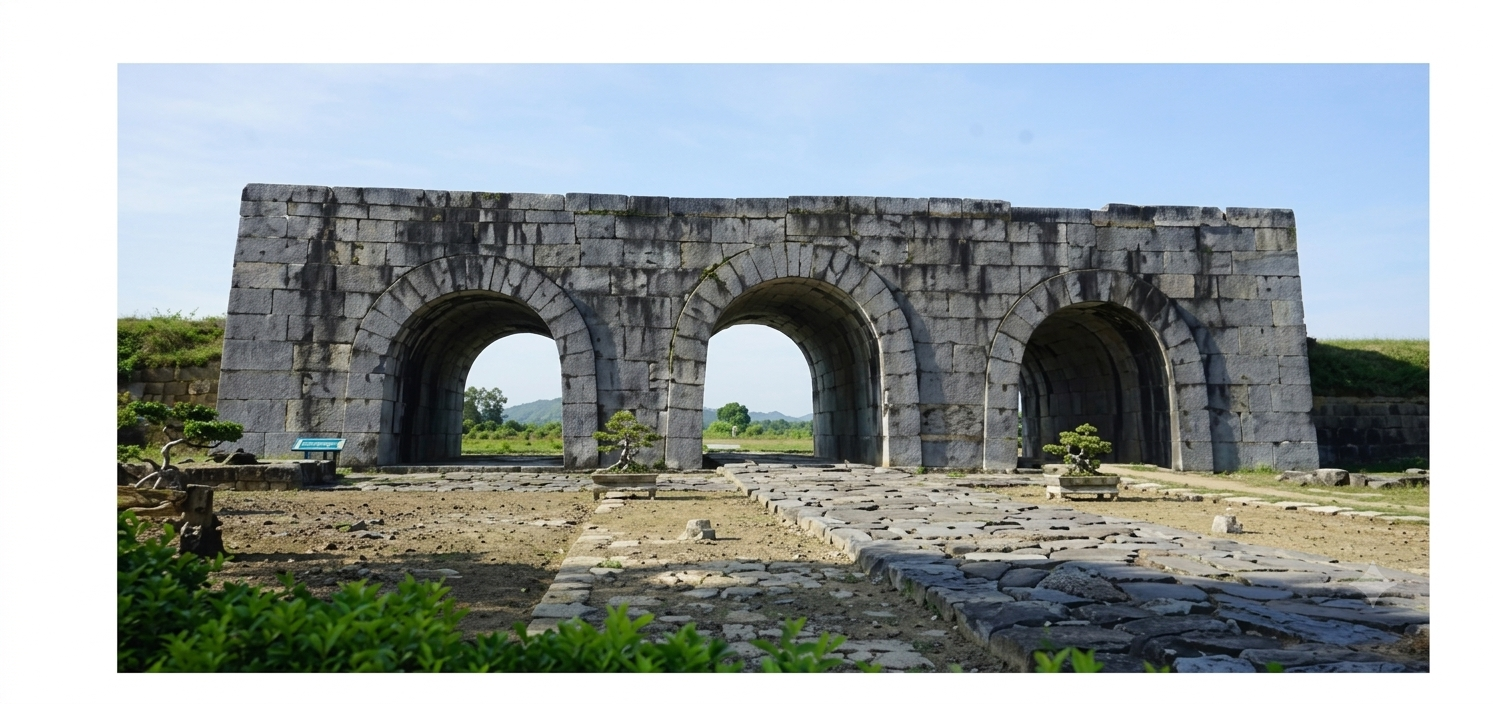
\includegraphics[width=0.4\textwidth]{../images/Thanh.png}
\end{figure}
}{
    \textbf{a)} & Chiều cao từ mặt đất đến đỉnh cửa là 5,75m.
    & \textcolor{amberorange}{$\bigcirc$} & \textcolor{amberorange}{$\bigcirc$} \\ \hline
    
    \textbf{b)} & Với hệ trục tọa độ Oxy đã chọn, đỉnh cửa là điểm \( I(0; 3,75) \).
    & \textcolor{amberorange}{$\bigcirc$} & \textcolor{amberorange}{$\bigcirc$} \\ \hline
    
    \textbf{c)} & Với hệ trục tọa độ Oxy đã chọn, vòm cửa là một phần của đồ thị hàm số  
    \(y = \dfrac{-7}{8,52}x^2 + 5,75.\)
    & \textcolor{amberorange}{$\bigcirc$} & \textcolor{amberorange}{$\bigcirc$} \\ \hline
    
    \textbf{d)} & Trước đây, ở mỗi cửa có cánh cửa làm bằng gỗ, khi khép lại thì cửa được đóng kín. Diện tích cửa gỗ của cửa chính giữa là 26,68 \( m^2 \) (kết quả làm tròn đến hàng phần trăm của đơn vị \( m^2 \)).
    & \textcolor{amberorange}{$\bigcirc$} & \textcolor{amberorange}{$\bigcirc$} \\
}

\questionShortAnswer{0}{2}{Một vòng xuyến ở ngã tư thành phố Tam Điệp có dạng hình tròn đường kính \( AB = 6m \). Công ty cây xanh thiết kế phần trồng hoa giấy ở giữa hai đường parabol có trục đối xứng vuông góc với đường kính \( AB \) tại tâm của hình tròn và cắt \( AB \) tại điểm \( C, C' \) thỏa mãn \( BC = 2m \) (phần tô đậm). Phần còn lại của vòng xuyến thiết kế trồng hoa có các chi phí để trồng hoa giấy và hoa cúc lần lượt là 200 000 đồng/m² và 100 000 đồng/m². Hỏi chi phí để trang trí vòng xuyến theo thiết kế là bao nhiêu nghìn đồng (kết quả làm tròn đến hàng đơn vị)?

\begin{center}
\begin{tikzpicture}[scale=1.2, >=latex]
    \fill[pattern=north east lines, pattern color=black!80]
        plot[domain=-1:1, samples=100] (\x, {-2*\x*\x + 2}) --
        plot[domain=1:-1, samples=100] (\x, {2*\x*\x - 2}) -- cycle;

    % 2. Vẽ đường tròn bao ngoài (bán kính R = 2)
    \draw[thick] (0,0) circle (2);

    % 3. Vẽ đường kính AB
    \draw[thick] (-2,0) -- (2,0);

    % 4. Vẽ parabol úp (phía trên)
    \draw[thick, samples=100, domain=-1:1] 
        plot (\x, {-2*\x*\x + 2});

    % 5. Vẽ parabol ngửa (phía dưới)
    \draw[thick, samples=100, domain=-1:1] 
        plot (\x, {2*\x*\x - 2});

    % 6. Nhãn các điểm
    \node[left] at (-2,0) {\small $A$};
    \node[right] at (2,0) {\small $B$};
    \node[below left] at (-1,0) {\small $C'$};
    \node[below right] at (1,0) {\small $C$};
\end{tikzpicture}
\end{center}
}

\questionShortAnswer{0}{3}{Bác An lên kế hoạch làm một cái biển quảng cáo phẳng, có thiết kế là phần được tô màu đậm trong hình vẽ bên dưới. Đường cong \( (P) \) là một parabol có đỉnh là điểm \( F \), có trục đối xứng là \( FH \) và đi qua các điểm \( A, B \). Tứ giác \( ABCD \) là hình chữ nhật, \( AB = 6m, BC = 2m, EF = 5m, FH = 1m \). Bác An kí hợp đồng với công ty X với đơn giá là 1,2 triệu đồng/1 \( m^2 \). Hỏi số tiền mà bác An phải trả sau khi làm xong cái biển quảng cáo là bao nhiêu triệu đồng?
\begin{center}
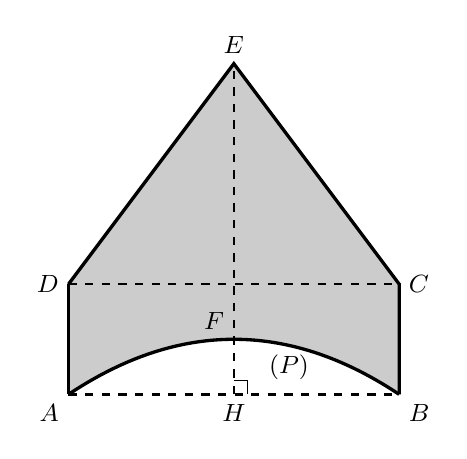
\begin{tikzpicture}[scale=0.7, >=latex]
    % 1. Tô màu xám phần biển quảng cáo
    \begin{scope}
        \fill[gray!40] 
            (-3,2) -- (0,6) -- (3,2) -- (3,0) -- 
            plot[domain=3:-3, samples=100] (\x, {-1/9*\x*\x + 1}) -- (-3,2) -- cycle;
    \end{scope}

    % 2. Đường nét đứt hỗ trợ
    \draw[thick, dashed] (-3,0) -- (3,0); % Đoạn AB
    \draw[thick, dashed] (-3,2) -- (3,2); % Đoạn CD
    \draw[thick, dashed] (0,0) -- (0,6);  % Trục EH qua F, H

    % 3. Khung viền phần tô đậm
    \draw[very thick] (-3,2) -- (0,6) -- (3,2) -- (3,0);
    \draw[very thick] (-3,2) -- (-3,0);
    \draw[very thick, samples=100, domain=-3:3] plot (\x, {-1/9*\x*\x + 1});

    % 4. Đánh dấu các góc vuông tại H
    \draw (0,0.25) -- (0.25,0.25) -- (0.25,0);

    % 5. Đánh dấu các tên điểm
    \node[below left] at (-3,0) {\small $A$};
    \node[below right] at (3,0) {\small $B$};
    \node[right] at (3,2) {\small $C$};
    \node[left] at (-3,2) {\small $D$};
    \node[above] at (0,6) {\small $E$};
    \node[above left] at (0,1) {\small $F$};
    \node[below] at (0,0) {\small $H$};
    \node[below] at (1, 0.9) {\small $(P)$};
\end{tikzpicture}
\end{center}
}



\questionShortAnswer{0}{4}{Ông An có một mảnh vườn hình Elip có độ dài trục lớn bằng \( 16 \, \text{m} \) và độ dài trục bé bằng \( 10 \, \text{m} \). Ông muốn trồng hoa trên một đai đất rộng \( 8 \, \text{m} \) và nhận trục bé của elip làm trục đối xứng (như hình vẽ). Biết kinh phí để trồng hoa là \( 100000 \, \text{đồng/1m}^2 \). Hỏi ông An cần bao nhiêu tiền để trồng hoa trên đai đất đó? (Số tiền được làm tròn đến hàng nghìn.)

\begin{center}
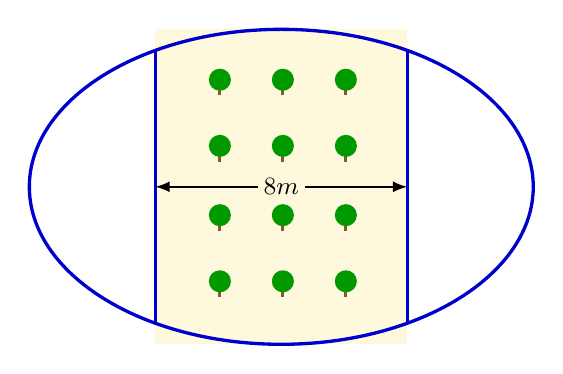
\begin{tikzpicture}[scale=0.4, >=latex]
    % Định nghĩa màu nền dải đất
    \definecolor{flowerland}{RGB}{254, 248, 220}

    % 1. Tô màu nền cho dải đất trồng hoa rộng 8m (x tư -4 đến 4)
    \begin{scope}
        \clip (-8,-5) rectangle (8,5);
        \fill[flowerland] (-4,-5) rectangle (4,5);
    \end{scope}

    % 2. Viền Elip chính
    \draw[very thick, blue!80!black] (0,0) ellipse (8 and 5);

    % 3. Viền dải đất dọc
    \begin{scope}
        \clip (0,0) ellipse (8 and 5);
        \draw[very thick, blue!80!black] (-4,-5) -- (-4,5);
        \draw[very thick, blue!80!black] (4,-5) -- (4,5);
    \end{scope}

    % 4. Mũi tên chỉ kích thước 8m
    \draw[<->, thick, black] (-4,0) -- (4,0) node[midway, fill=flowerland, inner sep=2pt] {\small $8\text{m}$};

    % 5. Minh họa biểu tượng cây/hoa đơn giản trong dải đất
    \foreach \x in {-2, 0, 2} {
        \foreach \y in {-3.2, -1.1, 1.1, 3.2} {
            \fill[brown!70!black] (\x, \y-0.3) rectangle (\x+0.1, \y);
            \fill[green!60!black] (\x+0.05, \y+0.2) circle (0.35);
        }
    }
\end{tikzpicture}
\end{center}
}

\end{document}